\documentclass[spanish]{beamer}

%Language symbols
\usepackage[spanish]{babel}
\selectlanguage{spanish}
\usepackage[utf8]{inputenc}
\usepackage{verbatim}


\usepackage{graphicx}% http://ctan.org/pkg/graphicx
\usepackage{caption,subcaption}

% Code

\usepackage{listings,textcomp}
\lstset{literate=   % listings config
  {á}{{\'a}}1 {é}{{\'e}}1 {í}{{\'i}}1 {ó}{{\'o}}1 {ú}{{\'u}}1
  {Á}{{\'A}}1 {É}{{\'E}}1 {Í}{{\'I}}1 {Ó}{{\'O}}1 {Ú}{{\'U}}1
  {à}{{\`a}}1 {è}{{\`e}}1 {ì}{{\`i}}1 {ò}{{\`o}}1 {ù}{{\`u}}1
  {À}{{\`A}}1 {È}{{\'E}}1 {Ì}{{\`I}}1 {Ò}{{\`O}}1 {Ù}{{\`U}}1
  {ä}{{\"a}}1 {ë}{{\"e}}1 {ï}{{\"i}}1 {ö}{{\"o}}1 {ü}{{\"u}}1
  {Ä}{{\"A}}1 {Ë}{{\"E}}1 {Ï}{{\"I}}1 {Ö}{{\"O}}1 {Ü}{{\"U}}1
  {â}{{\^a}}1 {ê}{{\^e}}1 {î}{{\^i}}1 {ô}{{\^o}}1 {û}{{\^u}}1
  {Â}{{\^A}}1 {Ê}{{\^E}}1 {Î}{{\^I}}1 {Ô}{{\^O}}1 {Û}{{\^U}}1
  {œ}{{\oe}}1 {Œ}{{\OE}}1 {æ}{{\ae}}1 {Æ}{{\AE}}1 {ß}{{\ss}}1
  {ű}{{\H{u}}}1 {Ű}{{\H{U}}}1 {ő}{{\H{o}}}1 {Ő}{{\H{O}}}1
  {ç}{{\c c}}1 {Ç}{{\c C}}1 {ø}{{\o}}1 {å}{{\r a}}1 {Å}{{\r A}}1
  {€}{{\EUR}}1 {£}{{\pounds}}1 {ñ}{{\~{n}}}1
}

\lstset{    %listings config
	language=C++,
	belowcaptionskip=1\baselineskip,
	breaklines=true,
	frame=L,
	xleftmargin=0.1in,
	%otherkeywords={},
	showstringspaces=false,
	backgroundcolor=\color{white},
	basicstyle=\footnotesize\ttfamily,
	keywordstyle=\bfseries\color{purple!90!black},
	commentstyle=\itshape\color{gray!85!},
	identifierstyle=\color{blue!80!black},
	stringstyle=\color{green!60!black},
}

%Theme
\usetheme{metropolis}

%Title
\title{Análisis de la eficiencia de algoritmos}
\date{\today}
\author{José Antonio Álvarez Ocete \\ Norberto Fernández de la Higuera \\ Javier Gálvez Obispo \\ Yábir García Benchakhtir}
\institute{Doble Grado en Ingeniería Informática y Matemáticas}
%Document
\begin{document}

\frame{\titlepage}

\begin{frame}\frametitle{Algoritmos de ordenación $O(n^2)$}

  \begin{itemize}
  \item Burbuja
  \item Insercción
  \item Selección
  \end{itemize}
\end{frame}

\begin{frame}
  El análisis teórico de este algoritmo nos dice que es $O(n^2)$

  $$\frac{a}{2} n^2 - \frac{3a}{2} n + a \in O(n^2)$$
\end{frame}

\begin{frame}\frametitle{Algoritmo burbuja}
  \begin{figure}[H]
    \centering   
        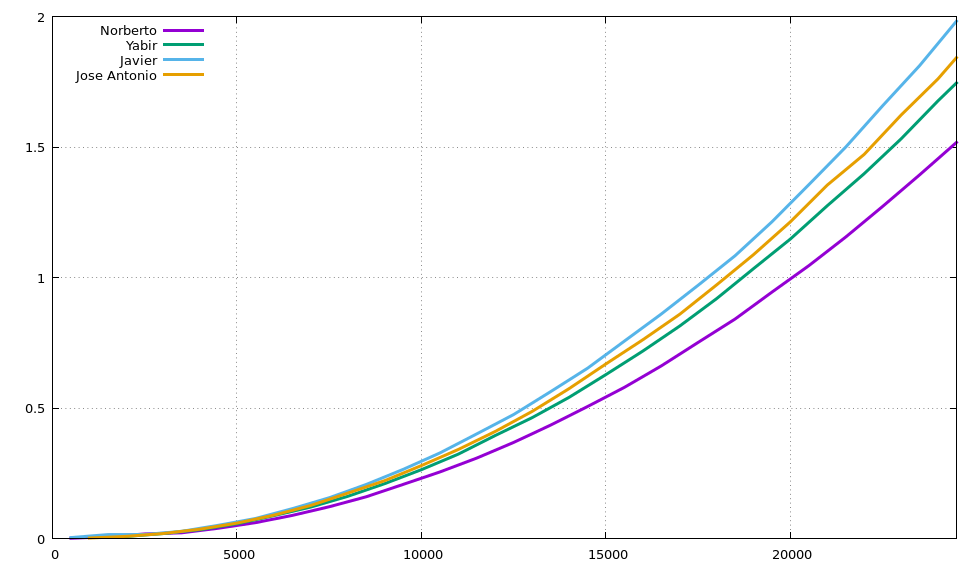
\includegraphics[clip,width=1\columnwidth]{../plots/burbuja.png}%
    \end{figure}
  \end{frame}

  \begin{frame}[fragile]\frametitle{Algoritmo de selección}

    \begin{lstlisting}
static void seleccion_lims(int T[], int inicial, int final) {
	int i, j, indice_menor;
	int menor, aux;
	for (i = inicial; i < final - 1; i++) {
		indice_menor = i;
		menor = T[i];
		for (j = i; j < final; j++) {
			if (T[j] < menor) {
				indice_menor = j;
				menor = T[j];
			}
		}
		aux = T[i];
		T[i] = T[indice_menor];
		T[indice_menor] = aux;
	};
}
\end{lstlisting}
    
\end{frame}

\begin{frame}\frametitle{Analizamos teóricamente este algoritmo}
  \begin{equation*}
  \begin{aligned}
    \sum_{i=0}^{n-1}\left[a_2 + \sum_{j=i}^n{a_1}\right] &= \sum_{i=0}^{n-1}\left[a_2+a_1\sum_{j=i}^{n}1\right]  \\
    &= \sum_{i=0}^{n-1}a_2 + a_1 \sum_{i=0}^{n}\sum_{j=i}^{n-1}1 \\
    &= a_2\sum_{i=0}^{n-1}1 + a_1 \sum_{i=0}^{n}(n-i)
  \end{aligned}
\end{equation*}
\end{frame}

\begin{frame}
  \begin{equation*}
  \begin{aligned}
    a\sum_{i=0}^{n-1}(n-i) &= a_1\left[\sum_{i=0}^{n}n - \sum_{i=0}^{n}i\right]  \\
    &= an^2 - a \frac{(n+1)n}{2} \\
    &= an^2- \frac{an^2}{2} - \frac{an}{2}
  \end{aligned}
\end{equation*}
\end{frame}

\begin{frame}
  Finalmente sumando las dos partes obtenemos:

  $$\frac{an^2}{2} - \frac{an}{2}+ b(n-1) = \frac{a}{2}n^2+\frac{b-a}{2}n - b \in O(n^2)$$
\end{frame}

\begin{frame}\frametitle{Algoritmo de selección}
  \begin{figure}[H]
    \centering   
        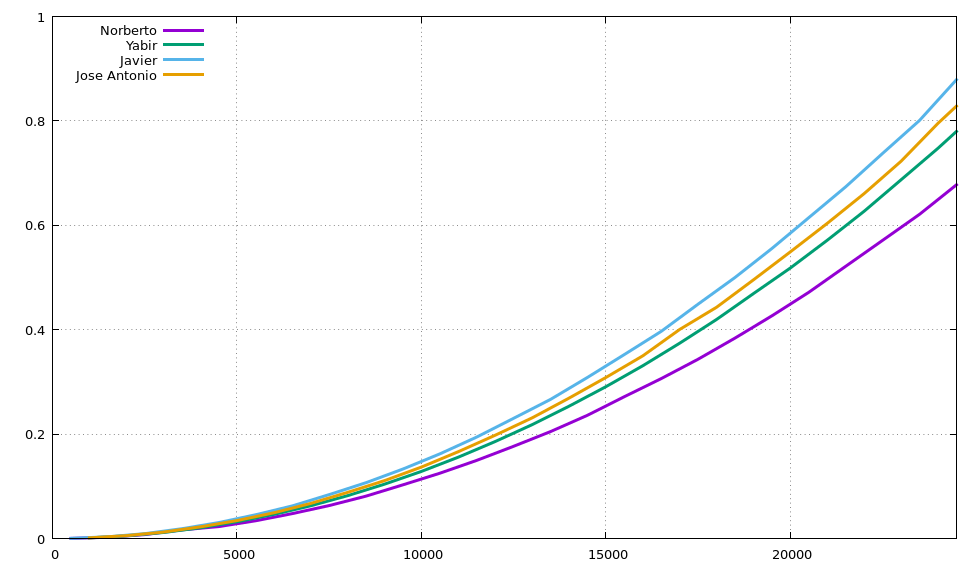
\includegraphics[clip,width=1\columnwidth]{../plots/seleccion}%
    \end{figure}
  \end{frame}

  \begin{frame}[fragile]\frametitle{Algoritmo de inserción}

\begin{lstlisting}
static void insercion_lims(int T[], int inicial, int final)
{
	int i, j;
	int aux;
	for (i = inicial + 1; i < final; i++) {
		j = i;
		while ((T[j] < T[j-1]) && (j > 0)) {
			aux = T[j];
			T[j] = T[j-1];
			T[j-1] = aux;
			j--;
		};
	};
}
\end{lstlisting}

\end{frame}

\begin{frame}
  $$\sum_{i=0}^{n} \sum_{j=i}^{n} a = ... = a \cdot (\frac{n^2}{2} + 2n) \in O(n^2)$$
\end{frame}


\begin{frame}\frametitle{Algoritmo de inserción}
  \begin{figure}[H]
    \centering   
        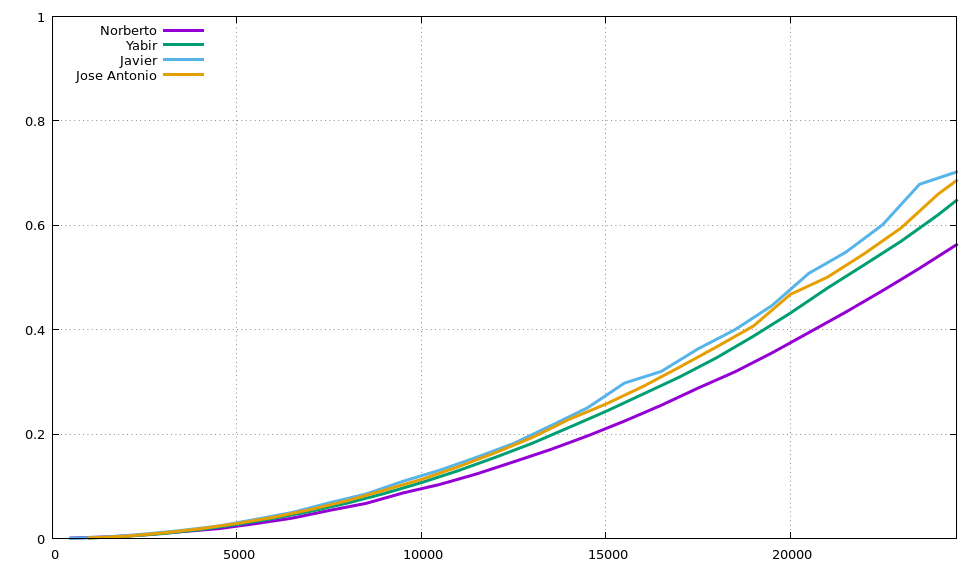
\includegraphics[clip,width=1\columnwidth]{../plots/insercion}%
    \end{figure}
  \end{frame}

  \begin{frame}\frametitle{Algoritmos de ordenación $O(nlog(n)$}

    \begin{itemize}
    \item mergesort
    \item heapsort
    \item quicksort
    \end{itemize}
    
\end{frame}

\begin{frame}\frametitle{Algoritmo mergesort}

  Como se ha visto en teoría la eficiencia de este algoritmo es:

  $$c_1n + c_2nlog_2(n) \in O(nlog_2(n))$$
  
\end{frame}

\begin{frame}
    \begin{figure}[H]
    \centering   
        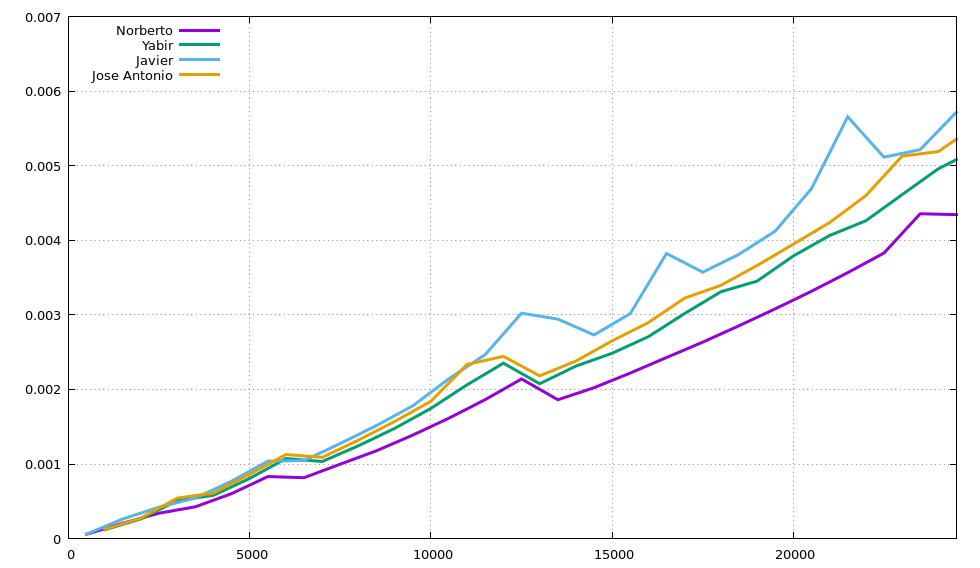
\includegraphics[clip,width=1\columnwidth]{../plots/mergesort}%
    \end{figure}
\end{frame}

\begin{frame}\frametitle{Algoritmo heapsort}

  \begin{lstlisting}
static void reajustar(int T[], int num_elem, int k) {
	int j;
	int v;
	v = T[k];
	bool esAPO = false;
	while ((k < num_elem/2) && !esAPO) {
		j = k + k + 1;
		if ((j < (num_elem - 1)) && (T[j] < T[j+1]))
			j++;
		if (v >= T[j])
			esAPO = true;
		T[k] = T[j];
		k = j;
	}
	T[k] = v;
}
\end{lstlisting}
  
\end{frame}
 
\end{document}